\documentclass[12pt,a4paper]{article}
\usepackage[T2A]{fontenc}
\usepackage[utf8]{inputenc}
\usepackage[english,russian]{babel}
\ifx\pdfoutput\undefined
	\usepackage{graphicx}
\else
	\usepackage[pdftex]{graphicx}
	\usepackage{epstopdf}
\fi
\usepackage{amssymb}
\usepackage{amsmath}
\usepackage[font=normalsize,labelfont=bf]{caption}
\usepackage[unicode=true, hypertexnames=false]{hyperref}
\usepackage{afterpage}
\hypersetup{
		pdftitle={Богданов Д.А., “Численное исследование теплового потока для задачи обтекания затупленного тела гиперзвуковым потоком ионизированного газа”, 2015},
    colorlinks,
    citecolor=black,
    filecolor=black,
    linkcolor=black,
    urlcolor=black
    }
\oddsidemargin=0pt
\textwidth=155mm
\title{Численное исследование теплового потока для задачи обтекания затупленного тела гиперзвуковым потоком ионизированного газа}
\author{Дмитрий Богданов}
\author{Сергей Поняев}
\date{}
\renewcommand\normalsize{\fontsize{14pt}{24pt}\selectfont}
\begin{document}
\renewcommand\normalsize{\fontsize{12pt}{14pt}\selectfont}
\begin{titlepage}
	\begin{center}
		\small{МИНИСТЕРСТВО ОБРАЗОВАНИЯ И НАУКИ \\ РОССИЙСКОЙ ФЕДЕРАЦИИ \\
Санкт-Петербургский государственный политехнический университет \\
Физико-механический факультет \\
Кафедра гидроаэродинамики}\\
		\vspace{0.18\textheight}
	\end{center}
	\begin{center}
		\vspace{0.1\textheight}
		\large{Численное исследование течения в фильтре-циклоне}\\
		\vspace{0.01\textheight}
		\normalsize
		\textsc{Автореферат диссертации на соискание ученой степени магистра по направлению 010600 – Прикладные математика и физика}
		\vspace{0.25\textheight}
	\end{center}
	\begin{minipage}{0.48\textwidth}
		\begin{flushleft}
			Выполнил студент гр. 6054/11\\
			Руководитель, к.ф.-м.н., с.н.с.\\
		\end{flushleft}
	\end{minipage}
	\begin{minipage}{0.5\textwidth}
		\begin{flushright}
			Богданов Д.А. \\
			Поняев С.А. \\
		\end{flushright}
	\end{minipage}
	\vspace{0.1\textheight}
	\begin{center}
		Санкт-Петербург \\
		\the\year
	\end{center}
\end{titlepage}
\newpage
\renewcommand\normalsize{\fontsize{14pt}{24pt}\selectfont}
\tableofcontents
\newpage
\section*{Введение}
	\subsection*{Актуальность проблемы}
		\hspace{1em} 	Задача очищения атмосферного воздуха от загрязняющих выбросов промышленных предприятий достаточно актуальна. Выбросы от стационарных источников вредных веществ в атмосферу городов и населенных пунктов, расположенных на территории северо-западного федерального округа,  по данным Росстата за 2007 год,  составили 2319000 тонн, в том числе твёрдых -- 289400 тонн \cite{emissionInfoRussian}. В некоторых отраслях промышленности доля выбросов пыли в атмосферу достигает 15\% от общего числа получаемого продукта. Так, при изготовлении одной тонны цемента в воздух выбрасывается $\approx 160$ кг цементной пыли \cite{emissionInfoEurope}.
		\begin{figure}[ht]
			\begin{minipage}{0.46\linewidth}
				\vspace{-1em}
				Динамика изменения объёма выбросов твёрдых вредных веществ в атмосферу \textit{(рис. \ref{figure:atmosphereDynamic})} имеет тенденцию к росту, что говорит о том, что решение проблемы инженерной защиты воздуха от вредных веществ останется актуальной и в ближайшем будущем. 
			\end{minipage}
			\hspace{0.01\linewidth}
			\begin{minipage}{0.48\linewidth}
				\centering
				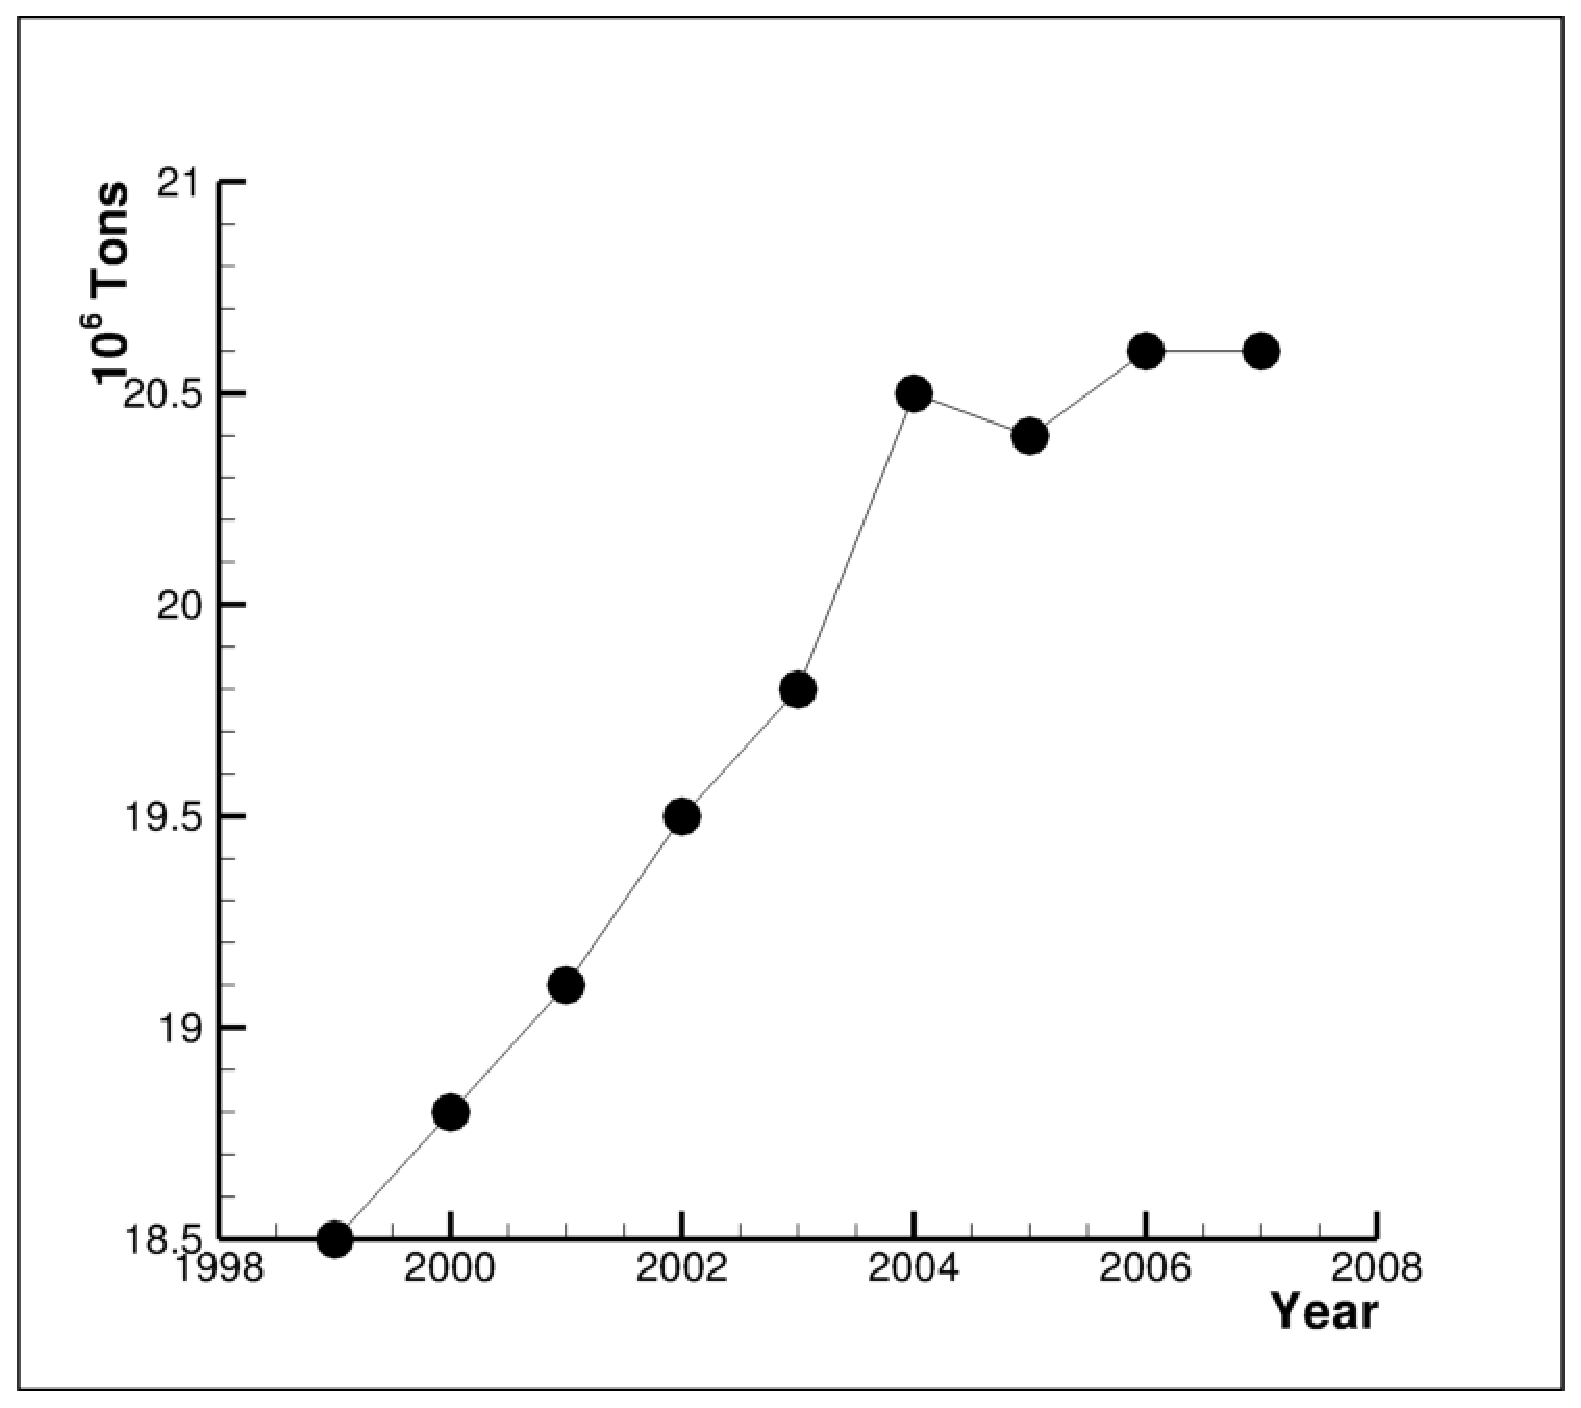
\includegraphics[scale=0.23]{atmosphereDynamic}
				\caption{Динамика выбросов твёрдых веществ в атмосферу \cite{emissionInfoRussian}}
				\label{figure:atmosphereDynamic}
			\end{minipage}
		\end{figure}
		\vspace{-1em}
	
		Для очищения воздуха от твёрдых примесей широкое распространение получили фильтры типа циклон. Циклон представляет собой инерционный пылеуловитель, в котором выделение частиц из воздушной среды происходит, в основном, под действием центробежной силы, возникающей при вращении воздушного потока в корпусе аппарата.
	
		Запылённый воздух входит в циклон через тангенциальный патрубок и, приобретая вращательное движение, опускается винтообразно вниз вдоль внутренних стенок цилиндра и конуса. Небольшая часть этого потока, в котором сконцентрированы пылевые частицы, движется в непосредственной близости от стенок циклона и поступает через пылеотводящее отверстие в пылесборный бункер, где происходит осаждение и накопление пылевых частиц.
	
		В центральной зоне циклона воздушный поток, освобождённый от пыли, поднимается винтообразно вверх и удаляется через выхлопную трубу наружу.
	
		Вследствие вращательного движения воздушного потока в центральной зоне циклона (в конусе, выхлопной трубе и пылесборном бункере) наблюдается пониженное давление.\cite{instructions}
	
		В силу высокой степени закрученности потока, необходимо введение поправок в модели турбулентности для учёта кривизны линий тока. Кроме того, учитывая высокую концентрацию частиц в потоке, в инженерных расчётах необходимо учитывать не только влияние потока на частицы, но также и обратное влияние частиц на поток.
	%Актуальность проблемы
	\subsection*{Цели работы}
		\begin{enumerate}
			\item Реализация $k-\omega-SST$ модели турбулентности с поправкой на кривизну линий тока при помощи открытой интегрируемой платформы для численного моделирования задач механики сплошных сред OpenFOAM.
			\item Реализация с использованием OpenFOAM солвера, имеющего в основе модель идеального газа и учитывающего при этом обратное влияние частиц на поток.
			\item Численное моделирование циклона с учётом обратного влияния частиц на поток и поправки на кривизну линий тока к генерации турбулентности.
		\end{enumerate}
	%Цели работы
%Введение

\newpage
\section{Обзор существующих исследований}
	Циклоны используются для удаления твёрдых частиц из газовых потоков с конца 19 века. Простая конструкция, низкие затраты на производство и обслуживание, а также адаптивность к широкому диапазону рабочих параметров сделали циклоны одними из наиболее часто используемых промышленных фильтров. 
	
		Эффективность циклонов определяется степенью очистки воздуха $\eta$, равной отношению количества частиц данного диаметра, задержанных циклоном к полному числу частиц. В силу того, что принцип работы этих фильтров основан на инерциальных силах, они имеют низкую эффективность для частиц, диаметром менее $5 \mu m$.
	
	Существует огромное количество конфигураций, однако противоточные циклоны с тангенциальным входом \textit{(рисунок \ref{fig:cycloneOverview})} чаще всего используются для очистки воздуха в промышленности. Такая конфигурация описывается девятью безразмерными параметрами \textit{(таблица \ref{tableCyclone})}, отнесёнными к масштабу длины $D$, характеризующему диаметр фильтра \cite{DirgoLeith}.\\
  \begin{minipage}{0.6\textwidth}
    \captionof{table}{Геометрия фильтра}
			\begin{tabular}{l l}
				\hline
				\label{tableCyclone}
				Диаметр цилиндра, & $D$\\
				Диаметр выходной трубы, & $D_e$\\
				Высота входного канала, & $a$\\
				Ширина входного канала, & $b$\\
				Длина выходной трубы, & $h_e$\\
				Полная высота фильтра, & $H$\\
				Высота цилиндра, & $h$\\
				Диаметр нижнего сечения фильтра, & $B$\\
				Высота пылесборника, & $h_d$\\
				Диаметр пылесборника, & $D_d$\\
			\end{tabular}
    \end{minipage}
    \hspace{1em}
  \begin{minipage}{0.35\textwidth}
    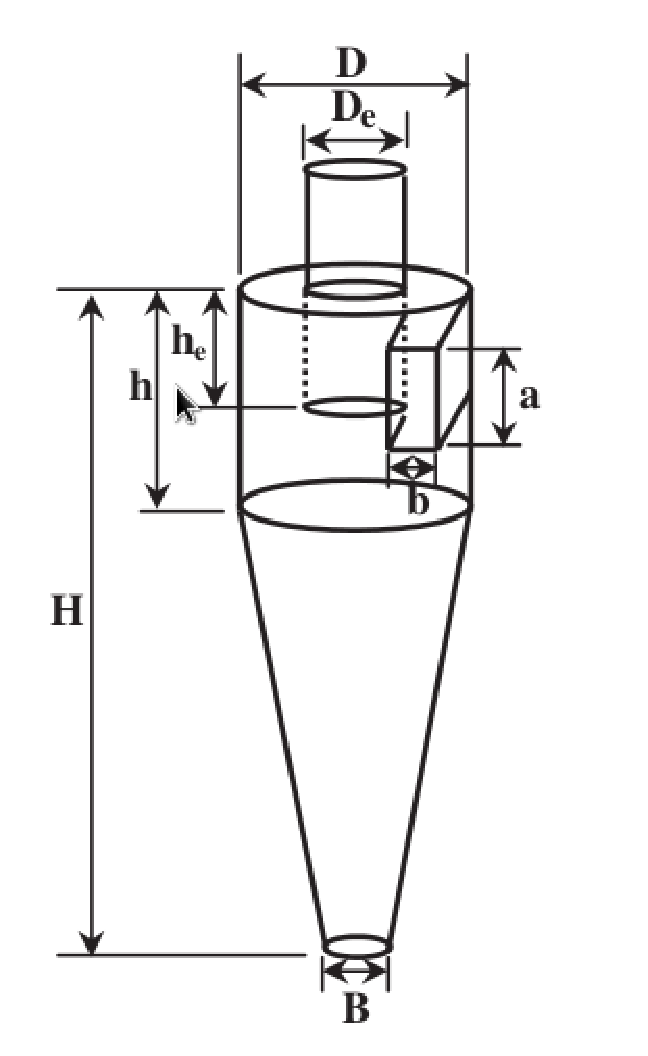
\includegraphics[scale=0.375]{Geometry}
				\captionof{figure}{Схема фильтра}
			    \label{fig:cycloneOverview}
  \end{minipage}
  	\subsection{Теоретические исследования}
	\label{theoreticalOverview}
		\hspace{1em}
		Процесс взаимодействия частиц с несущей фазой очень хорошо описан в книге \cite{Richardson}. Указанная книга предоставляет в явном виде решение большого количества инженерных задач, связанных с течениями дисперсных сред. В конечном виде эти решения являются в большой степени приближёнными, применимы в ограниченном числе случаев и описывают, в основном, общие параметры системы, не давая информации о структуре течения несущей фазы, фокусируясь именно на описании частиц. Тем не менее, теоретические модели, сформулированные в этой книге охватывают широкий диапазон физических процессов, связанных с течениями жидкостей с дисперсными включениями, и могут быть крайне полезны для математического описания таких течений.
		\subsubsection*{Степень очистки}
		\addcontentsline{toc}{subsubsection}{Степень очистки}
		Диргоу и Лейт \cite{DirgoLeith} в своей статье систематизировали теоретические модели, применяемые для расчётов рабочих параметров системы, выделив три основных подхода к описанию циклонов.
			\subparagraph{I. Подход, основанный на времени полёта частиц\\}
			Допустим, частица попадает в циклон на определённом расстоянии от оси фильтра. Частица должна переместиться из этого положения к стенке для того, чтобы быть отфильтрованной. Критический диаметр частицы это такой диаметр, при котором частица перемещается ровно на это расстояние за время пребывания в циклоне. Различные заключения о начальном положении частицы и времени пребывания приводят к различным приближённым решениям. Теория Лэппла \cite{Lapple} является наиболее часто используемым примером такого подхода. Предположим, что пыль, поступающая в циклон, равномерно распределена по всему входному сечению. Лэппл определил критический диаметр частиц для циклонов как диаметр, при котором, частицы, перемещаясь от середины входного сечения до стенки, за время пребывания в циклоне фильтруются с 50\% эффективностью:
			\begin{equation}
				\label{LappleEquation}
				d_{50} = \sqrt{\frac{9\mu b}{2 \pi \rho_p U_i C_d N_t}},
			\end{equation}
			где $\rho_p$ - плотность частиц, $U_i$ - скорость газа на входе в циклон, $\mu$ - динамическая вязкость воздуха, $b$ - ширина входного сечения фильтра, $C_d$ - коэффициент сопротивления.
			
	Число оборотов $N_t$, которые совершает газ внутри фильтра, может быть рассчитано по формуле $N_t = tU_i/\pi D$, а время пребывания $t$ равно отношению объёма циклона к объёмному расходу воздуха $Q$ \cite{Kuo}.
	
	Эффективность для частицы произвольного диаметра $d$ может быть определена из величины отношения этого диаметра к $d_{50}$.
	\begin{figure}[ht]
		\centering
		\includegraphics[scale=0.5]{Lapple}
		\caption{Степень очистки в зависимости от $d/d_{50}$}
		\label{fig:lapple}
	\end{figure}
	На \textit{рисунке \ref{fig:lapple}} показана степень очистки в зависимости от $d/d_{50}$, построенная на основе экспериментов Лэппла. Теодоре и де Паола \cite{Theodore} предлагают для определения степени очистки воздуха использовать следующее соотношение, определённое на основе экспериментов Лэппла:
			\begin{equation}
				\eta = \frac{1}{1 + (d/d_{50})^{-2}}
			\end{equation}
			\subparagraph{II. Подход, основанный на статике частиц\\}
			При таком подходе критический диаметр определяется как диаметр частицы, при котором действующая на частицу центробежная сила полностью компенсируется силой сопротивления. Такие частицы должны бесконечно вращаться вокруг границы ядра фильтра, расположенного под выходным сечением. Сила сопротивления, действующая на более мелкие частицы превышает центробежную силу так, что такие частицы пересекают эту границу и, поднимаясь наверх, вылетают из циклона. Более крупные частицы относятся к стенкам циклона и могут, таким образом, быть отфильтрованы. При таком определении критического диаметра, степень фильтрации растёт от нуля для частиц меньше критического диаметра до единицы для частиц, диаметром больше критического. На практике такое строгое разделение недостижимо из-за флуктуаций скорости, а эффективность для критического диаметра, в среднем, должна быть равной 50\%.
			
			Примером этого подхода может служить теория, предложенная в статье Барта \cite{Barth}. Барт определил границы ядра циклона, как воображаемое продолжение стенок выходной трубы до нижнего сечения фильтра или стенок конуса. При таком определении границы, критическая скорость для осаждения статических частиц выражается формулой
			\begin{equation}
				U^{*}_{ts} = \frac{Qg}{2 \pi h^{*} U^2_t}
			\end{equation}
			Степень очистки для других диаметров частиц определяется через отношение критической скорости произвольных частиц к критической скорости статических частиц
			\begin{equation}
				\frac{U_{ts}}{U^{*}_{ts}} = \frac{\pi h^{*}U^2_t\rho_p d^2}{9 \mu Q},
			\end{equation}
			где $h^{*}$ - высота ядра циклона, которая может быть найдена из геометрических соображений, а $Q$ - расход воздуха через входное сечение фильтра. Тангенциальная скорость газа на границе ядра, определяется, как 
			\begin{equation}
				U_t = U_o\left(\frac{(D_e/2)(D-b)\pi}{2ab\alpha + h^{*}(D-b)\lambda \pi}\right),
			\end{equation}
			где $\lambda = 0.02$ - коэффициент трения, $\alpha = 1-1.2(b/D)$, $U_o$ - скорость газа в выходном сечении, $a$ и $b$ - соответственно, высота и ширина входного сечения \cite{Barth}.
			\begin{figure}[ht]
				\centering
				\includegraphics[scale=0.48]{Barth}
				\caption{Степень очистки в зависимости от $U_{ts}/U^{*}_{ts}$}
				\label{fig:barth}
			\end{figure}
			На \textit{рисунке \ref{fig:barth}} показана зависимость степени очистки от $U_{ts}/U^{*}_{ts}$, построенная Бартом на основе экспериментальных результатов для нескольких конфигураций циклона. Кривая Барта хорошо аппроксимируется выражением
			\begin{equation}
				\eta = \frac{1}{1+ (U_{ts}/U^{*}_{ts})^{-3.2}}
			\end{equation}
	
			\subparagraph{III. Прямой расчёт эффективности очистки\\}

			Последний подход позволяет рассчитать эффективность очистки для любого размера частиц и любой конфигурации циклонов. Кривая степени очистки может быть определена без использования обобщённых кривых, основанных на критическом диаметре. Примерами такого подхода являются теория Лейта-Лихта \cite{LeithLicht} и теория Диетца \cite{Dietz}.
			
			Течение в промышленных циклонах на практике всегда является турбулентным. Модель Лейта-Лихта учитывает влияние турбулентности предполагая, что на любой высоте внутри циклона неосевшая пыль представляет собой равномерную смесь. Среднее время пребывания в циклоне определяется на основе его геометрических размеров и расходе воздуха. Итоговое выражение для степени очистки циклона выглядит следующим образом:
			\begin{equation}
				\eta = 1 - \exp[-2 (C\Psi)^{1/(2n+2)}].
			\end{equation}
			Влияние свойств частиц и газа учитывается в модифицированном инерционном параметре $\Psi$.
			\begin{equation}
				\Psi = \frac{\rho_p d^2 U_i (n+1)}{18 \mu D}.
			\end{equation}
			Здесь $C$ - безразмерный геометрический параметр, который зависит только от конфигурации фильтра:
			\begin{equation}
				\begin{aligned}
					\label{geometricParameterEfficiency}
					&C = \frac{\pi D^2}{ab} \Bigg[ 2 \left\lbrace 1 - \left( \frac{D_e}{D}\right)^2 \right\rbrace\left( \frac{h_e}{D} - \frac{a}{2D} \right) + \\ &+ \frac{1}{3} \left( \frac{h_e + l - h}{D} \right)\left( 1+\frac{d_c}{D} + \frac{d_c^2}{D^2}  \right) + \frac{h}{D} - \left( \frac{D_e}{D} \right)^2\frac{l}{D} - \frac{h_e}{D}\Bigg]			
				\end{aligned}
			\end{equation}
			Истинная длина циклона, $l$ определяется как максимальное расстояние, которое преодолевает вращающийся поток в зоне под выходной трубой. 
			\begin{equation}
				\label{naturalLength}
				l = 2.3D_e\left(\frac{D^2}{ab}\right)^{1/3}.
			\end{equation}
			Диаметр конуса на истинной длине определяется, как
			\begin{equation}
			\label{diameterAtNaturalLength}
				d_c = D - \frac{(D-B)(h_e + l -h)}{H - h}
			\end{equation}
			Если истинная длина превышает $(H-h_e)$, $l$ в уравнениях (\ref{geometricParameterEfficiency}) и (\ref{diameterAtNaturalLength}) заменяется на $(H - h_e)$.
			
			Степень экспоненты, $n = 0.5 \div 0.9$, определяет изменение тангенциальной скорости в радиальном направлении: $U_tr^n = const$. Эмпирическая формула для определения $n$ при произвольном диаметре циклона и заданной температуре газа выглядит следующим образом \cite{Alexander}:
			\begin{equation}
				\label{incrementN}
				n = 1 - \left[ (1-0.67D^{0.14})(T/283)^{0.3} \right]
			\end{equation}
			
			Модель Диетца \cite{Dietz} является модифицированным вариантом модели Лейта-Лихта. Диетц разделяет циклон на три региона -- входной участок, область опускающегося течения и ядро циклона. Предполагается, что под действием турбулентности устанавливается равномерный в радиальном направлении профиль концентрации неотфильтрованных частиц внутри каждого региона. Предполагается также, что происходит обмен частицами между областью опускающегося течения и ядром циклона. Для расчёта эффективности циклона предлагается формула
			\begin{equation}
				\eta = 1 - \left[ K_0 - \sqrt{K_1^2 + K_2^2} \right]\exp{\left[\frac{-\pi (2h_e - a)\rho_p d^2 U_i}{18 \mu ab}\right]},
			\end{equation}
			где 
			\begin{eqnarray}
				K_0 &=& \frac{1}{2}\left[ 1 + \left(\frac{D_e}{D}\right)^{2n}\left(1+\frac{9\mu ab}{ \pi \rho_p l d^2 U_i}\right) \right] \\
				K_1 &=& \frac{1}{2}\left[ 1 - \left(\frac{D_e}{D}\right)^{2n}\left(1+\frac{9\mu ab}{ \pi \rho_p l d^2 U_i}\right) \right] \\
				K_2 &=& \left(\frac{D_e}{D}\right)^{2n}.
			\end{eqnarray}
			Как и в модели Лейта-Лихта, $l$ должна быть заменена на $(H-h_e)$, если $l>(H-h_e)$. Величина $n$ может быть вычислена по формуле (\ref{incrementN}).
	\subsubsection*{Перепад давления}
	\addcontentsline{toc}{subsubsection}{Перепад давления}
		Величина перепада давления, создаваемого циклоном, являясь показателем необратимых потерь энергии, имеет чрезвычайно важное значение, поскольку она непосредственно связана с эксплуатационными расходами. Перепад давления определяется, как разница давлений между входным и выходным сечениями фильтра \cite{Utikar}. Циклоны в этом плане имеют одну важную особенность, которая заключается в наличии радиальной компоненты скорости в выходном сечении фильтра, которая затрудняет определение статического давления в этой области. На практике, разница давлений между входной и выходной границей ниже, чем истинный перепад давления.
		
		Обобщенный вариант формулы для определения давления представляет собой произведение числа Эйлера на скоростной напор:
		\begin{equation}
			\triangle P_{air-only}  = \frac{16ab}{D_e^2} \left( \frac{\rho_g U_i^2}{2} \right).
		\end{equation}
		Для слабо запылённых потоков уравнение записанное с использованием безразмерных геометрических параметров, предложенное Лэпплом является более надёжным:
		\begin{equation}
			\triangle P_{air-only} = \frac{16\left(\frac{a}{D}\right)\left(\frac{b}{D}\right)}{\left(\frac{D_e}{D}\right)^2} \frac{\rho_g U_i^2}{2} = \frac{16\left(\frac{a}{D}\right)\left(\frac{b}{D}\right)}{\left(\frac{D_e}{D}\right)^2}\left(\frac{\rho_g\left(\frac{Q}{ab}\right)^2}{2}\right).
		\end{equation}
		Примечательно, что перепад давления сначала падает с увеличением концентрации дисперсных включений, а потом снова начинает расти, начиная с некоторой, достаточно большой, концентрации примесей \cite{Shrikant}. Для определения перепада давления с учётом концентрации примеси используется уравнение Смольника \cite{Smolik}
		\begin{equation}
			\triangle P_{with-solids} = \triangle P_{air-only} (1-0.02c^{0.6}),
		\end{equation}
		где $c$ - концентрация твёрдых частиц на входе в циклон.
	\subsection{Экспериментальные исследования}
		\hspace{1em}Существует большое количество работ по экспериментальному исследованию течения с искривлёнными линиями тока. Среди них стоит выделить достаточно подробный эксперимент, приведённый в статье Monson et al. \cite{Monson}. Авторы статьи проводят численное и экспериментальное исследование турбулентного течения воздуха в U-образном канале.
		
		Экспериментальному моделированию циклонов также уделено немало внимания. Среди статей, приводящих экспериментальные данные по турбулентному течению в циклонах, можно, опять же, отметить детальное исследование течения в циклоне модели Stairmand, описанное в статье J. Dirgo, D. Leith \cite{DirgoLeith}. В этой статье приведены данные для профилей скорости в нескольких сечениях фильтра для большого диапазона рабочих параметров. К сожалению, авторы используют модифицированную модель фильтра, в которой масштаб $D = 0.375m$ отличается от классического $D = 0.205m$, предложенного в работе Stairmand \cite{Stairmand}, поэтому экспериментальные данные неприменимы к моей работе, в которой рассматривается именно классическая модель фильтра.
	\subsection{Численные исследования}
		\hspace{2em}Численному моделированию течения в циклонах посвящено очень много инженерных исследований.
	%Численные исследования
\newpage
%Обзор существующих моделей

\newpage
<<<<<<< HEAD
\section*{Заключение}
\addcontentsline{toc}{section}{Заключение}

В ходе исследования была рассмотрена задача о турбулентном течении газа с дисперсными включениями в фильтре-циклоне при разных значениях скорости потока и различных диаметрах частиц.

Для проведения расчётов в OpenFOAM был имплементирован поправочный коэффициент Шура-Спалларта для учёта влияния кривизны линий тока на турбулентные характерестики. Верификация модели производилась на задаче о турбулентном течении воздуха в U-образном канале и показала явный положительный эффект на результаты расчётов по сравнению с немодифицированной SST-моделью. Результаты расчётов хорошо согласуются с экспериментальными данными Монсона.

Расчёт циклона также показал положительное влияние введённой поправки на профили скорости. 

Сравнение результатов расчётов, выполненных при помощи введённого в OpenFOAM солвера и Fluent показало отличное соответствие решений друг другу. Анализ влияния дисперсных включений на основной поток позволил заключить, что этим влиянием в исследуемой задаче, по большому счёту, можно пренебречь.

Проведено сравнение результатов расчётов с экспериментальными данными Диргоу и Лейта для степени очистки, которое показало хорошее согласие как с экспериментами, так и с теорией, которую эти эксперименты подтверждают. Показана эффективность циклонов для очищения газа от твёрдых частиц диаметром $\sim 10^{-6}m$. Выявлено, что при уменьшении скорости течения, эффективность рассматриваемой конфигурации циклона заметно понижается. Такая же закономерность имеет место и при уменьшении диаметра частиц. Выяснено, что для фильтрации частиц, диаметром меньше $\approx 10^{-7}m$, циклон непригоден так как степень очистки при этом становится меньше 30\%.
=======
%!TEX root = Dissertation.tex
>>>>>>> pif/master

    \newpage
\thispagestyle{plain}
\bibliographystyle{unsrt}
\bibliography{dimbib}
\end{document}